\def\difficulty{2}
\sujet{Freeman Chain Code}

\begin{note}This tutorial is focused on shape representation by the Freeman chain code. This code is an ordered sequence of connected segments (of specific sizes and directions) representing the contour of the shape to be analyzed. The direction of each segment is encoded by a number depending on the selected connectivity (Fig. \ref{fig:freeman:chaincode}). In this example, the contour of the shape and its Freeman code are given in 4-con\-nec\-ti\-vi\-ty.	
\end{note}

\index{Topology!Neighborhood}
\index{Freeman Chain Code}
\begin{figure}[htbp]
\centering\caption{Freeman chain code examples.}%
\subfloat[4-connected\newline neighborhood.]{\begin{tikzpicture} 
  \draw[->] (0,0) -- (1,0); 
\draw[->] (0,0) -- (-1,0); 
\draw[->] (0,0) -- (0,1); 
\draw[->] (0,0) -- (0,-1);

\node[below] at (1,0){0};
\node[below] at (-1,0){2};
\node[above] at (0,1){1};
\node[below] at (0,-1){3};
\end{tikzpicture}}
\hfill
\subfloat[Example Freeman code in a\newline 4-neighborhood.]{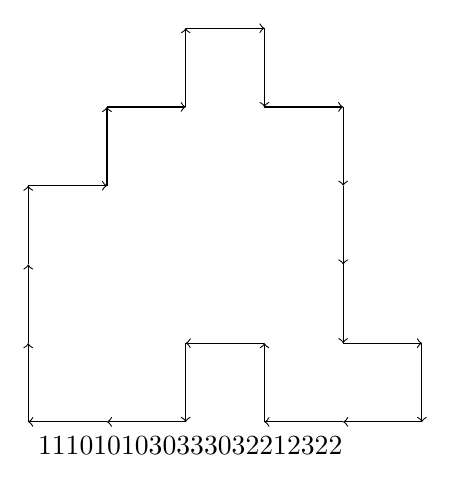
\begin{tikzpicture} 
\draw[->] (0,0)--(0,1);
\draw[->] (0,1)--(0,2);
\draw[->] (0,2)--(0,3);
\draw[->] (0,3)--(1,3);
\draw[->] (1,3)--(1,4);
\draw[->] (1,4)--(2,4);
\draw[->] (2,4)--(2,5);
\draw[->] (2,5)--(3,5);
\draw[->] (3,5)--(3,4);
\draw[->] (3,4)--(4,4);
\draw[->] (4,4)--(4,3);
\draw[->] (4,3)--(4,2);
\draw[->] (4,2)--(4,1);
\draw[->] (4,1)--(5,1);
\draw[->] (5,1)--(5,0);
\draw[->] (5,0)--(4,0);
\draw[->] (4,0)--(3,0);
\draw[->] (3,0)--(3,1);
\draw[->] (3,1)--(2,1);
\draw[->] (2,1)--(2,0);
\draw[->] (2,0)--(1,0);
\draw[->] (1,0)--(0,0);

\node[right] at (0,-.3) {1110101030333032212322};
\end{tikzpicture}}
\hfill
\subfloat[8-connected\newline neighborhood.]{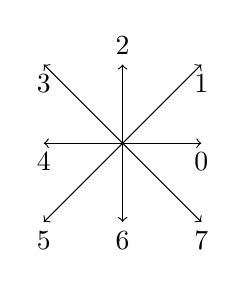
\begin{tikzpicture} 
  \draw[->] (0,0) -- (1,0); 
\draw[->] (0,0) -- (-1,0); 
\draw[->] (0,0) -- (0,1); 
\draw[->] (0,0) -- (0,-1);

  \draw[->] (0,0) -- (1,1); 
\draw[->] (0,0) -- (-1,1); 
\draw[->] (0,0) -- (-1,-1); 
\draw[->] (0,0) -- (1,-1);

\node[below] at (1,0){0};
\node[below] at (-1,0){4};
\node[above] at (0,1){2};
\node[below] at (0,-1){6};

\node[below] at (1,1){1};
\node[below] at (-1,1){3};
\node[below] at (1,-1){7};
\node[below] at (-1,-1){5};
\end{tikzpicture}}
%\begin{center}\includegraphics{chain_code.jpg}  \end{center}
\label{fig:freeman:chaincode}%
\end{figure}


\noindent \textbf{Notations:}
\begin{itemize}
	\item  $y$ is 4-adjacent to $x$ if $|y_1-x_1|+|y_2-x_2|\leq 1$.
	\item  $y$ is 8-adjacent to $x$ if $\max(|y_1-x_1|,|y_2-x_2|)\leq 1$.
	\item $N_4(x)=\{y:y\text{ is 4-adjacent to } x\}$; $N_4^*(x)=N_4(x)\backslash \{x\}$.
	\item $N_8(x)=\{y:y\text{ is 8-adjacent to } x\}$; $N_8^*(x)=N_8(x)\backslash \{x\}$.
\end{itemize}

{
	\makeatletter
	\renewcommand\fs@ruled{\def\@fs@cfont{\bfseries}\let\@fs@capt\floatc@ruled
		\def\@fs@pre{\hrule height.8pt depth0pt \kern2pt}%
		\def\@fs@post{\kern2pt\hrule\relax}%
		\def\@fs@mid{\vskip2pt}%
		\let\@fs@iftopcapt\iftrue}
	\makeatother
\begin{figure}[H]
\centering
\subfloat[$V_4(x)$]{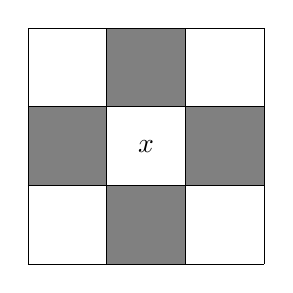
\begin{tikzpicture}
\fill[gray] (1,0) rectangle (2,1);
\fill[gray] (2,1) rectangle (3,2);
\fill[gray] (0,1) rectangle (1,2);
\fill[gray] (1,2) rectangle (2,3);
\draw[step=1cm,black,very thin] (0,0) grid (3,3);
\node  at (1.5,1.5) {$x$};
\end{tikzpicture}
} \hspace*{1.5cm}
\subfloat[$V_8(x)$]{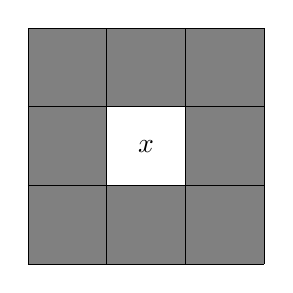
\begin{tikzpicture}
\fill[gray] (0,0) rectangle (3,1);
\fill[gray] (0,1) rectangle (1,2);
\fill[gray] (0,2) rectangle (3,3);
\fill[gray] (2,1) rectangle (3,2);
\draw[step=1cm,black,very thin] (0,0) grid (3,3);
\node  at (1.5,1.5) {$x$};
\end{tikzpicture}
}
\end{figure}
}
%

\section{Shape contours}
\index{Characterization}
Before determining the Freeman chain code of the shape, it is necessary to extract its contour.
\begin{qbox}
\begin{enumerate}
	\item Generate or load a simple shape as a binary image $A$.
	\item Extract its contour $C_4(A)$ ou $C_8(A)$ according to the 4-con\-nectivity or the 8-con\-nectivity, respectively:
	
	\begin{eqnarray*}
	x\in C_4(A)&\Leftrightarrow&\exists y\in N_8(x)\quad y\in {^c}\!A\\
	x\in C_8(A)&\Leftrightarrow&\exists y\in N_4(x)\quad y\in {^c}\!A
	\end{eqnarray*}
	 
\end{enumerate}
\end{qbox}

\begin{mcomment}
 \begin{mhelp}
  You can use the function \minline{bwperim} with the appropriate connectivity number.
 \end{mhelp}

\end{mcomment}

\begin{pcomment}
 \begin{phelp}
  You can erode the object and subtract this erosion to it, with a structuring element that corresponds to $N_4$ or $N_8$ if you want to have 8 or 4 connectivity, respectively.
 \end{phelp}

\end{pcomment}


\section{Freeman chain code}
From the shape contours, the Freeman chain code can be calculated.
\begin{qbox}
\begin{enumerate}
	\item From the binary array of pixels, extract the first point belonging to the shape (from left to right, top to bottom).
	
	\begin{pcomment}
	 \begin{phelp}
	  You can use \pinline{np.argwhere} to locate the first point.
	 \end{phelp}

	\end{pcomment}
	
	\begin{mcomment}
	 \begin{mhelp}
	  You can use \minline{find} to locate the first point.
	 \end{mhelp}

	\end{mcomment}


	\item From this initial point, determine the Freeman chain code $c$ (counterclockwise direction) using the $N_4$ or $N_8$ connectivity.
\end{enumerate}
\end{qbox}

\section{Normalization}
The Freeman chain code is depending on the initial point and is not invariant to shape rotation. It is then necessary to normalize this code.
\begin{enumerate}
	\item The first step consists in defining a differential code $d$ from the code $c$ :
	\begin{eqnarray*}
		d_k=c_k-c_{k-1} (\text{mod 4 or 8})
	\end{eqnarray*}
	In this example, $d=3003131331300133031130$;
	\item The second step consists in normalizing the code $d$. We have to extract the lowest number $p$ from all the cyclic translations of $d$.\\
	In this example, $p=0013303113030031313313$.\\
	 This Freeman chain code $p$ is then independant from the initial point and invariant by rotations of angles $k*\pi/2$ radians ($k\in \mathbb{Z}$).
	 
\end{enumerate}
\begin{qbox}
 \begin{itemize}
  \item Code above steps 1 and 2. Prototypes of functions are given.
  \item Validate your code by rotating the shape of $3\pi/2$ radians.
 \end{itemize}

\end{qbox}

	\begin{pcomment}
\begin{python}
def codediff(fcc, connectivity=8):
# computes differential code
\end{python}


\begin{premark}
 Use \pinline{numpy.roll} for circularly shifting the freeman code array. Code a small function that tests all elements of array, one by one, in order to get the minimum of two arrays.
\end{premark}

	\end{pcomment}
	
	\begin{mcomment}
\begin{matlab}
function d=codediff(fcc,conn)
\end{matlab}

\begin{mremark}
 Use \minline{circshift} for circularly shifting the freeman code array.
 Use \minline{polyval} for transforming the array of values into a number, although rounding errors might occur, due to numerical approximation of floating numbers.
\end{mremark}
\end{mcomment}



\section{Geometrical characterization}
\subsection{Perimeter}
From the Freeman chain code, it is possible to make different geometrical measurement of the shape.
\begin{qbox}Calculate the perimeter of the shape (take care of the diagonals).
	
	
	\end{qbox}
	
\subsection{Area}
The area is evaluated by the following algorithm:
\begin{itemize}
	\item The area is initialized to  $0$ and the parameter $B$ is initialized to $0$.
	\item For each iteration on the Freeman chain code $c$, the area and the para\-me\-ter va\-lue $B$ are incremented with the following rules:
	
	\begin{center}
	\begin{tabular}{|c|c|c|}
	\hline
		8-code & area & $B$\\\hline
		0&-B&0\\
		1&-B-0.5&1\\
		2&0&1\\
		3&B+0.5&1\\
		4&B&0\\
		5&B-0.5&-1\\
		6&0&-1\\
		7&-B+0.5&-1\\\hline
	\end{tabular}
	\end{center}
\end{itemize}
\begin{qbox}
Calculate the area of the shape in 8-con\-nec\-ti\-vity. Note that the area does not correspond to the total number of pixels belonging to the shape.
\end{qbox}

